\begin{figure}[!t]
\centering
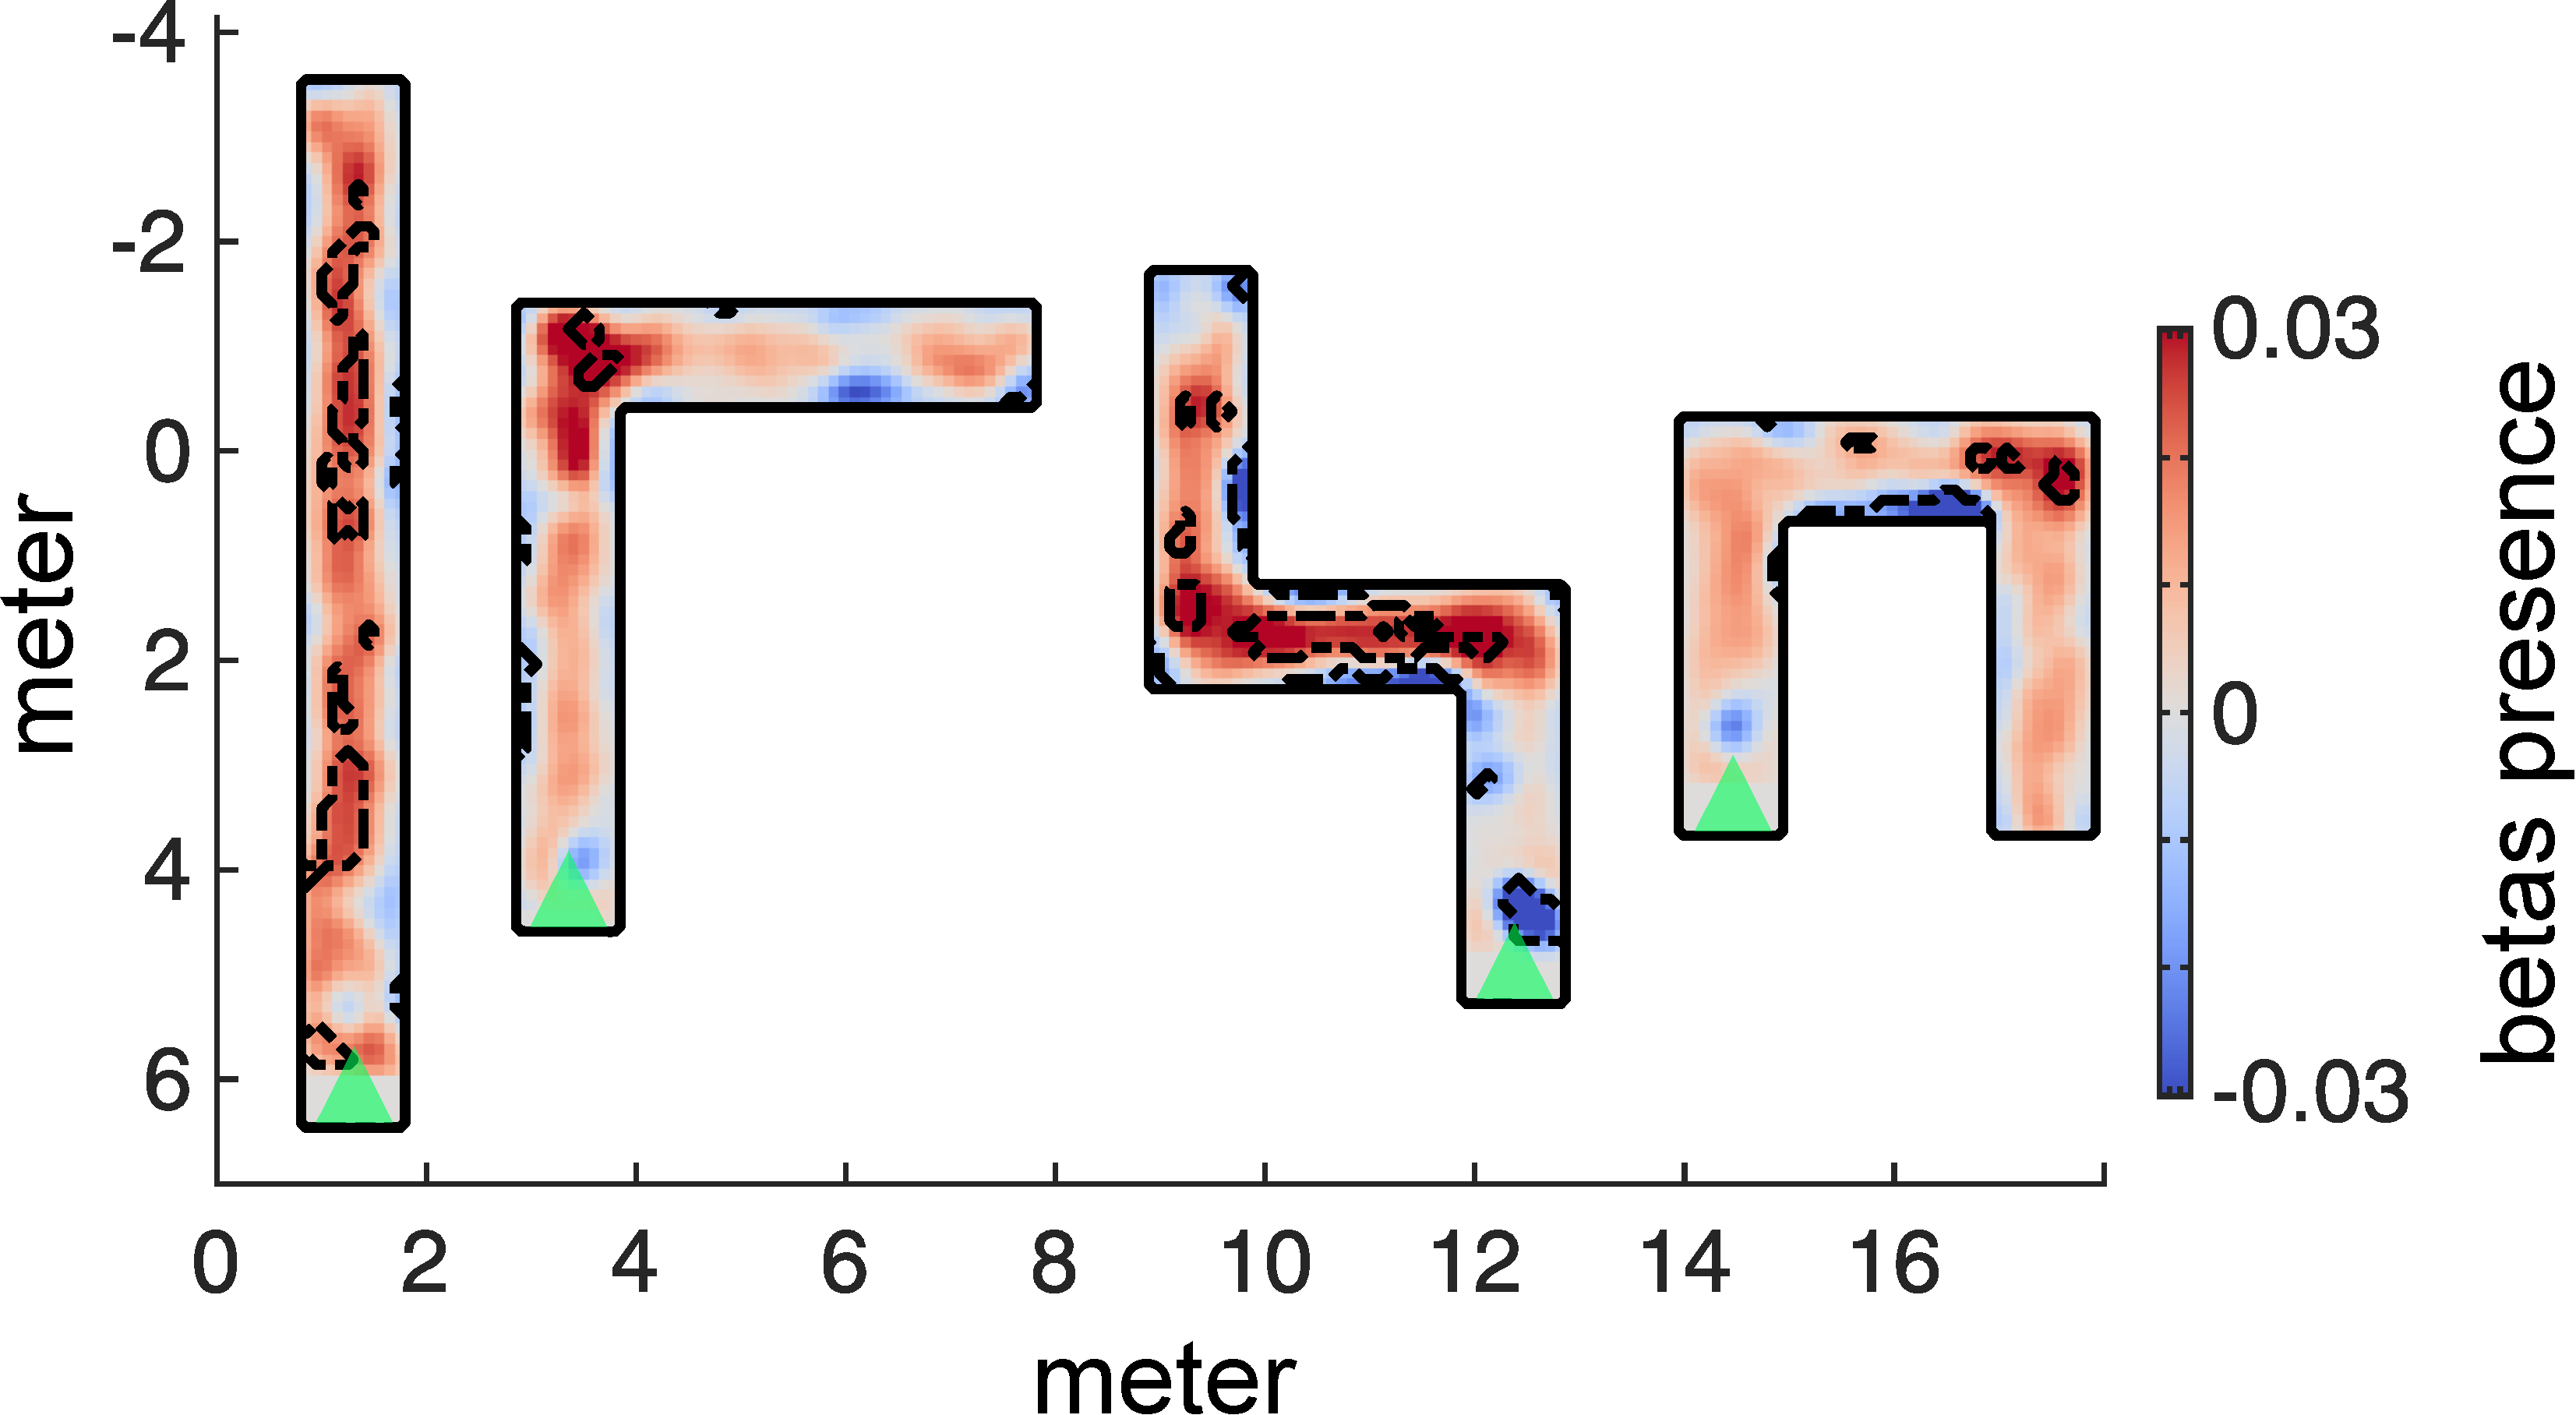
\includegraphics[width=\linewidth]{figures/head_loc_reg.pdf}
\caption{Map of the impact of presence on the time spent at every location in each of the four mazes: I, L, Z, U. Warmer colors refer to a positive regression estimate. For easy readability we introduce the reasoning for a positive estimate: for each 1 point increase in reported presence, participants stayed z seconds longer at location xy.}
\label{presence_head_loc}
\end{figure}

\subsection{Video game experience, biological sex and perspective taking predict presence experience} A step-wise model selection resulted in three predictors remaining, explaining 53,4\% of the variation in experienced presence ($F_{(3,25)}=11.69, p < .001,$ adjusted $R^2=.534$). Participants' predicted presence was equal to $8.15 - 1.2 (Video Game Experience) + 2.61 (Biological Sex) - 0.02 (PTSOT)$ where biological sex was dummy-coded as 0 = Male, 1 = Female, increasing video game experience was coded with higher scores and decreasing perspective taking ability with higher scores. Video game experience ($t_{(25)}=-4.7, p<.001$), biological  sex ($t_{(25)}=5.6, p<.001$) as well as perspective taking ability ($t_{(25)}=-2.52, p=.02$) were significant predictors of presence. Cross-validation of the three predictor model above yielded a combined average .76 mean absolute error. Hence, using video game experience, biological  sex as well as perspective taking ability we were able to predict experienced presence to within three-quarters of a point accuracy on the `IPQ Likert scale'.


%%%%% writing ressources
%Grand average number of touches at each location in each of the four mazes: I, L, Z, U. Hotter colors, i.e. redder, indicate a higher number of touches. Note, the location of each wall touch was located to where the participants head (VR Headset) was located at that time point, not its hand.
%Map of the impact of presence on the number of touches at every location in each of the four mazes: I, L, Z, U. Warmer colors refer to a positive regression estimate. For easy readability we introduce the reasoning for a positive estimate: for each 1 point increase in reported presence, participants touched the walls z times at location xy.